\documentclass[10pt,utf8]{beamer}
\usepackage[unicode]{hyperref}
\usepackage[T1]{fontenc}
\usepackage[polish]{babel}
\usepackage{bookman}
\usepackage{verbatim}

\usepackage{graphicx}
%Warsaw,Frankfurt,Rochester
\usetheme{Rochester} %motyw

\date{14 lutego 2013}

\linespread{1.5}
%Deklaracja kolorów
%\usecolortheme[rgb={0,0,0.5}]{structure}
\begin{document}
%
\title[System wsparcia procesu obsługi umów cywilno-prawnych - aplikacja w architekturze trójwarstwowej]{System wsparcia procesu obsługi umów cywilno-prawnych - aplikacja w architekturze trójwarstwowej}
\author{Konrad Miziński}
\institute{Instytut Informatyki \newline Politechnika Warszawska}
%

\begin{frame} %ramka, nie slajd!!!
\titlepage %strona tytulowa
\end{frame}
\begin{frame}
\tableofcontents
\end{frame}

\section{Wstęp}

\begin{frame}{Cel pracy}
	\subsection{Motywacja}
	Motywacja:
	\begin{itemize}
		\item Upowszechnienie umów cywilno-prawnych spowodowane kryzysem gospodarczym.
		\item Potrzeba stworzenia systemu obsługi umów w OKNO PW.
		\item Brak dedykowanych rozwiązań na rynku.
	\end{itemize}
\end{frame}
\begin{frame}{Cel pracy}
	\subsection{Cel pracy}
	Stworzenie prototypu systemu do wsparcia procesu obsługi umów cywilno-prawnych
	\begin{itemize}
		\item Zastosowanie architektury trójwarstwowej.
		\item Uwzględnienie specyfiki uczelni.
	\end{itemize}
\end{frame}

\section{Umowy cywilno-prawne}

\begin{frame}{Typy umów}
	\subsection{Typy umów}
	\begin{itemize}
		\item Umowa zlecenia
		\begin{itemize}
			\item najpopularniejsza forma umowy prawa cywilnego
			\item umowa starannego działania
			\item może być nieodpłatna
		\end{itemize}
		\item Umowa o dzieło
		\begin{itemize}
			\item umowa rezultatu
			\item zawsze odpłatna
		\end{itemize}
	\end{itemize}
\end{frame}


\begin{frame}{Postawa prawna}
	\subsection{Postawa prawna}
	Kodeks cywilny:
	\begin{itemize}
		\item art. 66-72 - Podstawowe regulacje
		\item art. 734-751 - Umowa zlecenia
		\item art. 627-646 - Umowa o dzieło
	\end{itemize}
	\vspace{\baselineskip}
	W przypadków umów cywilno-prawnych nie ma zastosowania Kodeks pracy!
\end{frame}

\begin{frame}{Zagadnienia dotyczące umów}
	\subsection{Zagadnienia dotyczące umów}
	\begin{itemize}[]
		\item Podatek dochodowy
		\item Koszty uzyskania przychodu
		\item Prawa autorskie
		\item Ubezpieczenia społeczne, ubezpieczenie zdrowotne, fundusze celowe
	\end{itemize}
\end{frame}

\section{Zrealizowana aplikacja}


\begin{frame}{Architektura aplikacji}
\subsection{Architektura aplikacji}
	\begin{center}
    Architektura trójwarstwowa z cienkim klientem
   \end{center} 	
	\begin{figure}[h]
    \begin{center}
    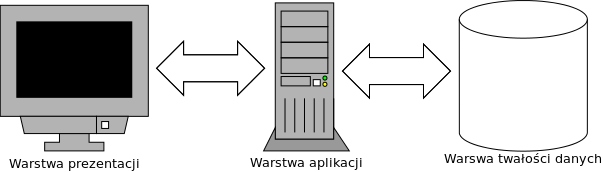
\includegraphics[angle=0,scale=0.4]{warstwy.png}
    \end{center} 
	\end{figure}
	\visible<0>{
		Warstwa trwałości danych 
		\begin{itemize}
			\item PostgreSQL
		\end{itemize}
	}
\vspace{\baselineskip}
\end{frame}


\begin{frame}{Architektura aplikacji}
	\begin{center}
    Architektura trójwarstwowa z cienkim klientem
   \end{center} 	
	\begin{figure}[h]
    \begin{center}
    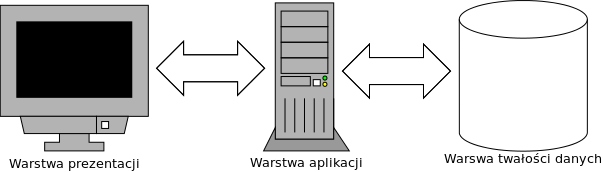
\includegraphics[angle=0,scale=0.4]{warstwy.png}
    \end{center} 
	\end{figure}
	\visible<1>{
		Warstwa trwałości danych 
		\begin{itemize}
			\item PostgreSQL
		\end{itemize}
	}
\vspace{\baselineskip}
\end{frame}


\begin{frame}{Architektura aplikacji}

Warstwa logiki biznesowej
		\begin{itemize}
			\item JEE
			\item ObjectLedge
			\begin{itemize}
				\item PicoContainer
				\item Velocity
				\item Ledge Intake
				\item Ledge Security
			\end{itemize}
			\item Hibernate
			\item wzorce DAO oraz POJO
		\end{itemize}
\end{frame}

\begin{frame}{Architektura aplikacji}
	Warstwa prezentacji
	\begin{itemize}
		\item HTML
		\item CSS
		\item JavaScript
		\item Dojo Toolkit
		\item AJAX
	\end{itemize}

\end{frame}

\begin{comment}
\begin{frame}{Wybrane funkcjonalności}
	\subsection{Wybrane funkcjonalności}	
	\begin{itemize}
		\item Umowy
		\begin{itemize}
			\item predefiniowane typy umów
			\item dowolne okresy płatności
			\item automatyczne generowanie rachunków
			\item wydruki do formatu pdf
		\end{itemize}
	\end{itemize}
	\begin{itemize}
		\item Pracownicy
		\begin{itemize}
			\item statusy pracowników z punktu widzenia ubezpieczeń społecznych
		\end{itemize}
	\end{itemize}
\end{frame}

\end{comment}

\begin{frame}{Wybrane funkcjonalności}	
	\subsection{Wybrane funkcjonalności}	
\begin{columns}
\begin{column}{5cm}
	\begin{itemize}
		\item Umowy
		\begin{itemize}
			\item predefiniowane typy umów
			\item dowolne okresy płatności
		\end{itemize}
	\end{itemize}
\end{column}
\begin{column}{5cm}
\begin{figure}[h]
    \begin{center}
    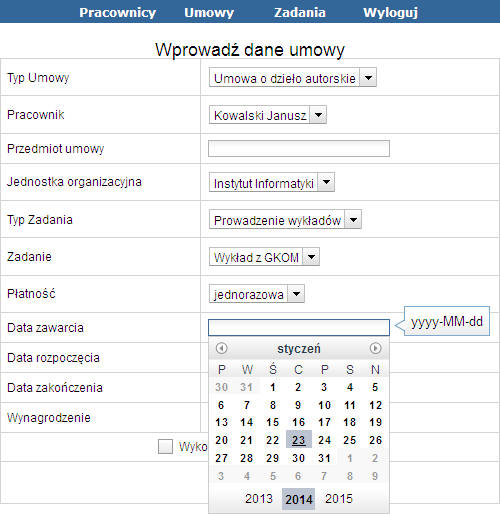
\includegraphics[angle=0,scale=0.4]{umowaForm.png}
    \end{center}
    
\end{figure}
\end{column}
\end{columns}
\end{frame}


\begin{frame}{Wybrane funkcjonalności}
	\begin{itemize}
		\item Umowy
		\begin{itemize}
			\item automatyczne generowanie rachunków
			\item wydruki do formatu pdf
		\end{itemize}
	\end{itemize}
\begin{figure}[h]
    \begin{center}
    
\includegraphics[angle=0,scale=0.45]{umowaPdf.png}
    \end{center}
    
\end{figure}
\end{frame}




\begin{frame}{Wybrane funkcjonalności}	
	\begin{columns}
		\begin{column}{5cm}
			\begin{itemize}
				\item Pracownicy
				\begin{itemize}
					\item statusy pracowników z punktu widzenia ubezpieczeń społecznych
				\end{itemize}
			\end{itemize}
		\end{column}
		\begin{column}{5cm}
			\begin{figure}[h]
    		\begin{center}
    			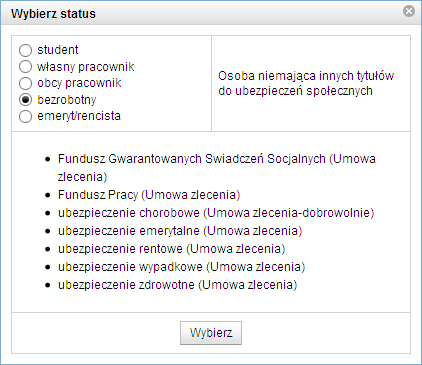
\includegraphics[angle=0,scale=0.5]{status.png}
    		\end{center}
			\end{figure}
\end{column}
\end{columns}
\end{frame}


\begin{frame}{Organizacja instytucji}
	\begin{figure}[h]
    \begin{center}
    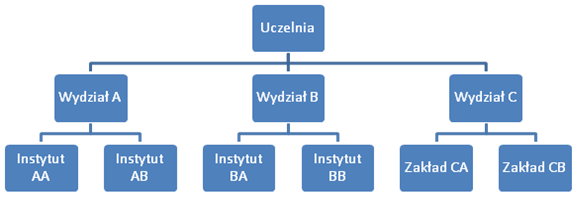
\includegraphics[angle=0,scale=0.7]{organizacja.png}
    \end{center} 
	\end{figure}
	\begin{itemize}
		\item Model hierarchiczny
		\item Odzwierciedlony w systemie bezpieczeństwa
		\item Zadania wykonywane w ramach jednostek
	\end{itemize}
\end{frame}

\section{Podsumowanie}
\begin{frame}{Podsumowanie}
	\begin{itemize}
		\item Cel pracy został osiągnięty
		\item Wstępna akceptacja przez OKNO PW
		\item Decyzja o dalszym rozwoju aplikacji
	\end{itemize}
\end{frame}

\begin{frame}
	\begin{center}
	\textbf{
	\LARGE
	Dziękuję za uwagę.
	}
	\end{center}
\end{frame}

\end{document}
